\documentclass[border=4pt]{standalone}
\usepackage{tikz,amsmath,amssymb}
\usetikzlibrary{arrows.meta,calc}
% Charte ENSTA
\definecolor{nuit}{HTML}{190F3C}\definecolor{bleu}{HTML}{3746FF}
\definecolor{bleuclair}{HTML}{9BA3FF}\definecolor{corail}{HTML}{FF808B}
\definecolor{corailf}{HTML}{D6455A}
\begin{document}
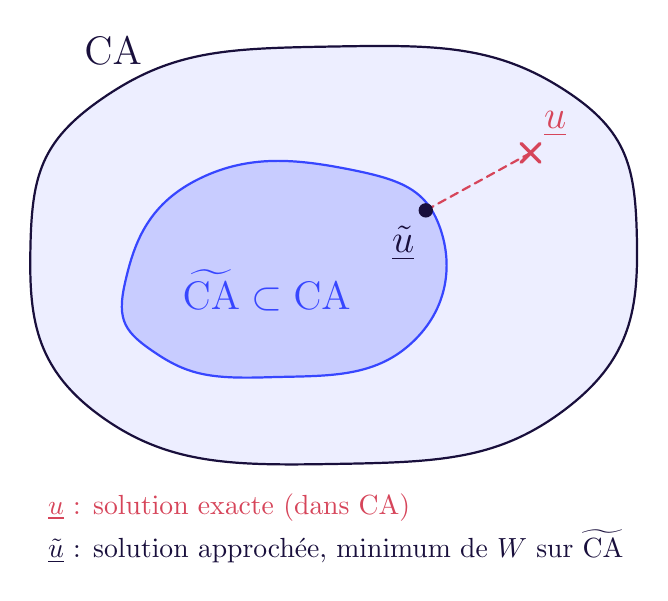
\begin{tikzpicture}[line cap=round,line join=round,>={Straight Barb[length=5pt]}]
  % Ensemble CA des champs cinématiquement admissibles
  \draw[thick,nuit,fill=bleuclair!18]
    plot[smooth cycle,tension=0.8] coordinates
      {(-3.6,0.2) (-2.6,2.1) (0.2,2.7) (3.1,2.2) (4.1,0.3) (3.2,-1.9) (0.3,-2.6) (-2.7,-2.0)};
  % Sous-ensemble restreint CA~ (dimension finie)
  \draw[thick,bleu,fill=bleuclair!55]
    plot[smooth cycle,tension=0.8] coordinates
      {(-2.4,-0.3) (-1.5,1.0) (0.4,1.15) (1.6,0.4) (1.2,-1.1) (-0.6,-1.5) (-2.0,-1.2)};
  % Étiquettes des ensembles
  \node[nuit] at (-2.55,2.65) {\Large $\mathrm{CA}$};
  \node[bleu] at (-0.6,-0.4) {\Large $\widetilde{\mathrm{CA}}\subset\mathrm{CA}$};
  % Solution exacte u (hors de CA~) et meilleure approximation u~ dans CA~
  \coordinate (u) at (2.75,1.35);
  \coordinate (ut) at (1.42,0.62);
  \draw[densely dashed,corailf,thick] (u) -- (ut);
  \draw[corailf,very thick] ($(u)+(-0.12,-0.12)$) -- ($(u)+(0.12,0.12)$)
                            ($(u)+(-0.12,0.12)$) -- ($(u)+(0.12,-0.12)$);
  \node[corailf,anchor=south west] at ($(u)+(0.05,0.08)$) {\Large $\underline{u}$};
  \fill[nuit] (ut) circle (2.6pt);
  \node[nuit,anchor=north east] at ($(ut)+(-0.02,-0.08)$) {\Large $\underline{\tilde{u}}$};
  % Légende (sous le schéma)
  \node[anchor=west,corailf] at (-3.5,-3.15) {$\underline{u}$ : solution exacte (dans $\mathrm{CA}$)};
  \node[anchor=west,nuit] at (-3.5,-3.65) {$\underline{\tilde{u}}$ : solution approchée, minimum de $W$ sur $\widetilde{\mathrm{CA}}$};
\end{tikzpicture}
\end{document}
